\tikzstyle{vertex}=[circle,fill=black,minimum size=10pt]
\tikzstyle{red vertex}=[circle,fill=red,minimum size=10pt]
\tikzstyle{blue vertex}=[circle,fill=blue,minimum size=10pt]
\tikzstyle{green vertex}=[circle,fill=green,minimum size=10pt]
\tikzstyle{grey vertex}=[circle,fill=yellow,minimum size=10pt]
\tikzstyle{edge} = [draw,line width=2pt]

\begin{figure}
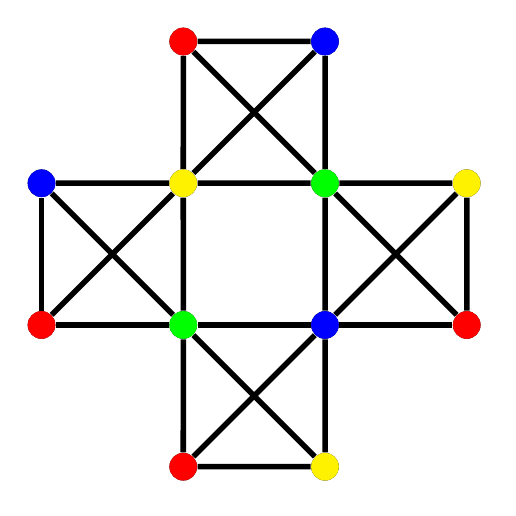
\begin{tikzpicture}[scale=1.8, auto,swap]
  \foreach \pos/\name in { {(0,0)/a},{(0,1)/b},{(1,0)/c},{(1,1)/d}, % Erstes Quadrat
                     {(1,2)/e},{(2,1)/f},{(2,2)/g}, % Zweites Quadrat
                     {(2,0)/h},{(1,-1)/i},{(2,-1)/j}, % Drittes Quadrat
                     {(3,0)/k},{(3,1)/l}} % Viertes Quadrat
                     \node<1->[vertex] (\name) at \pos {};
    % Connect vertices with edges and draw weights
        \foreach \source/ \dest in {a/b,a/c,a/d,b/c,b/d,c/d,e/f,e/g,e/d,f/g,f/d,d/g,h/i,h/j,i/j,c/h,c/i,c/j,h/f,h/k,h/l,f/k,f/l,k/l}
        \path<1->[edge] (\source) --  node{}  (\dest);
%
%    % Start animating the vertex and edge selection. 

        \foreach \pos in { {(0,0)},{(1,-1)},{(1,2)},{(3,0)}}
        \node<2->[red vertex] () at \pos{};
        \foreach \pos in { {(0,1)},{(2,2)},{(2,0)}}
        \node<3->[blue vertex] () at \pos{};
        \foreach \pos in { {(1,0)},{(2,1)}}
        \node<4->[green vertex] () at \pos{};
        \foreach \pos in { {(1,1)},{(2,-1)},{(3,1)}}
        \node<5->[grey vertex] () at \pos{};

%    % For convenience we use a background layer to highlight edges
%    % This way we don't have to worry about the highlighting covering
%    % weight labels. 
%    %\begin{pgfonlayer}{background}
%    %    \pause
%    %    \foreach \source / \dest in {d/a,d/f,a/b,b/e,e/c,e/g}
%    %        \path<+->[selected edge] (\source.center) -- (\dest.center);
%    %    \foreach \source / \dest / \fr in {d/b/4,d/e/5,e/f/5,b/c/6,f/g/7}
%    %        \path<\fr->[ignored edge] (\source.center) -- (\dest.center);
%    %\end{pgfonlayer}
\end{tikzpicture}
\end{figure}
